% Main body with filler text
\begin{figure*}[t!]
    \centering
    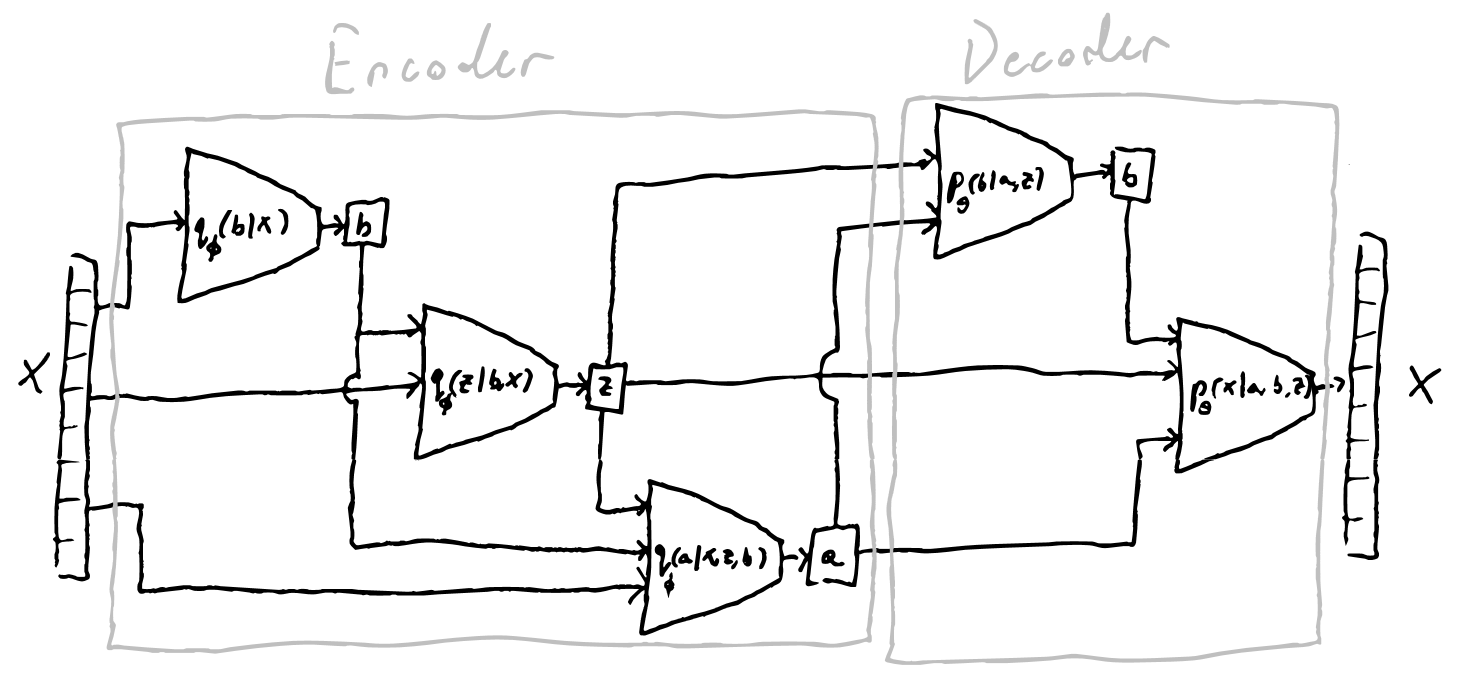
\includegraphics[width=\textwidth]{figures/model_sketch.png}
    \caption{Caption}
    \label{fig:sketch}
\end{figure*}

\section{PREDVAE}
\label{sec:methods}

% \subsection{Variational Autoencoders}
% \label{subsec:vae}

% A standard VAE, outlined in Fig. \textcolor{red}{[INSERT FIG]}, is composed of two neural networks referred to as the \textit{encoder} and the \textit{decoder}. The encoder is parameterized by $\boldsymbol{\theta}$ and maps an input vector $\mathbf{x}$ to a distribution over the lower-dimensional latent space, $q_{\boldsymbol{\theta}}(\mathbf{y}|\mathbf{x})$, where $\mathbf{y}$ denotes the latent space. The decoder is parameterized by $\boldsymbol{\phi}$ and takes as input samples $\mathbf{y}$ from the latent distribution. The aim of the decoder network is to learn a mapping from random samples of the latent space to the distribution over inputs, $p_{\boldsymbol{\phi}}(\mathbf{x}|\mathbf{y})$.

% \textcolor{red}{BLALBALBA SOMETHING SOMETHING ELBO AND VARIATIONAL INFERENCE.}

% The probabilistic nature of VAEs have proven to be a powerful tool for learning information-rich representations of inputs. The fact that distributions instead of point measures are learned allows for an expression of model uncertainty in the latent space. This feature means that VAEs are a viable tool for breaking degeneracies present in broad-band photometric observations lacking spectroscopic follow up, as is the case for photo-z estimation. \textcolor{red}{WRITE SOMETHING ABOUT THE DEGENERACY HERE, OR MENTION EARLIER?}

\subsection{Semi-Supervised Variational Autoencoders}
\label{subsec:ssvae}

Variational autoencoders (VAEs, first introduced by \cite{kingmaAutoEncodingVariationalBayes2022} and \cite{rezendeStochasticBackpropagationApproximate2014}, belong to a family of unsupervised neural networks that are trained to copy its input to its output in a probabilistic manner. This probabilistic mapping leads to a generative model that can be used to produce new samples from the input distribution. 
While VAEs have received attention in the past for their generative capabilities \textcolor{red}{[CITATIONS]}, their current utility stems from their ability to map a high-dimensional input into a lower dimensional compressed representation, known as the \textit{latent space}. In this setting VAEs have shown to be extremely competitive, being able to produce disentangled representations of complex inputs in a hierarchical manner \textcolor{red}{[INSERT REPRESENTATION LEARNING PAPERS FROM LOCAL ZOTERO]}. 

Although VAEs have been applied to astrophysical use-cases before to disentangle data \textcolor{red}{[INSERT SOME OF THE ASTRO VAE PAPERS]}, they have seen little use in photo-z estimation. This is most likely due to the unsupervised nature of VAEs, which can only indirectly be applied to the case of photo-z estimation by using latent representations of photometric observations as training data for a supervised ML model. In such an approach there is no assurance that the latent representations are optimal for the secondary supervised learning task \citep{kingmaSemiSupervisedLearningDeep2014}. Extensive work has been done in extending VAEs to the semi-supervised setting, jointly learning disentangled representations \textit{and} classifications of data \textcolor{red}{[CITE KINGMA 14, MAALØE 16, OTHERS?]}.

In this work we make use of such an extension, the \textit{Skip Deep Generative Model (SDGM)} introduced by \cite{maaløe}, which we review in this section. As inputs for the model we have observed data $\mathbf{X} = \mathbf{X}^p \cup \mathbf{X}^s$ where $\mathbf{X}^p = \{ \mathbf{x}_1,\dots,\mathbf{x}_{N_p} \}$ denotes the subset with only photometric data $\mathbf{x}_i$ available and $\mathbf{X}^s = \{ (\mathbf{x}_1, z_1), \dots , (\mathbf{x}_{N_s}, z_{N_s}) \}$ denotes the subset of the data with both photometric data and spectroscopic redshifts $z_i$. The SDGM assumes that the observed data is described by a generative model parameterized by a neural network with parameters $\theta$ 
\begin{align}
    p_\theta(x, z, a, b) = p_\theta(x|a,b,z) p_\theta(b|a,z) p(a) p(z).    
\end{align}
Here $p(a)$ and $p(z)$ are priors over an unobserved set of latent variables $a\in\mathbb{R}^A$ and the redshifts $z$ respectively, $p_\theta(b|a,z)$ is a neural network parameterizing the conditional distribution over a set of auxilliary latent variables $b\in\mathbb{R}^B$, and $p_\theta(x|a,b,z)$ is a neural network parameterizing the likelihood of $x$. The auxilliary latent variables $b$ allow for dependencies between the latent variables $a$ and redshifts $z$. This generative model corresponds to the decoder component in Fig. \ref{fig:sketch}.

Given this generative model, the target of optimization for $(x,z)\in \mathbf{X}^s$ is the marginal likelihood $p_\theta(x,z)$ with respect to the parameters $\theta$. This target is intractable due to the intractability of the posterior distribution $p(a,b|x,z)$. To solve this, the posterior distribution is approximated by a variational distribution $q_\phi(a,b|x,z)=q_\phi(a|b,x,z) q_\phi(b|x)$ parameterized by neural networks with parameters $\phi$, leading to a variational lower bound \textcolor{red}{CITE MAALØE}
\begin{align}
    \log p(x,z) &= \log \int_a \int_b p_\theta (x,z,a,b) dadb \\
    &\geq \mathbb{E}_{q_\phi(a,b|x,z)} \left[ \log \frac{p_\theta(x,z,a,b}{q_\phi(a,b|x,z)} \right] \\
    &= -\mathcal{S}(x,z). \label{eq:spec_loss}
\end{align}
For $x \in \mathbf{X}^p$ we instead optimize the marginal likelihood $p_\theta(x)$ with respect to $\theta$, where the redshift $z$ is now considered a latent variable. As before a variational distribution $q_\phi(a,b,z|x)=q_\phi(a|z,b,x)q_\phi(z|b,x)q_\phi(b|x)$ is introduced, leading to a variational lower bound
\begin{align}
    \log p(x) &= \log \int_a \int_b \int_z p_\theta (x,z,a,b) dadbdz \\
    &\geq \mathbb{E}_{q_\phi(a,b,z|x)} \left[ \log \frac{p_\theta(x,z,a,b}{q_\phi(a,b,z|x)} \right] \\
    &= -\mathcal{P}(x). \label{eq:phot_loss}
\end{align}
The conditional redshift distribution $q_\phi(z|b,x)$ appears in $-\mathcal{P}(x)$ but not $-\mathcal{S}(x,z)$. To improve the predictive accuracy over redshift an explicit likelihood term over observed spectroscopic redshifts is added,
\begin{align}
    \Tilde{\mathcal{S}}(x,z) = \mathcal{S} + \alpha \mathbb{E}_{q_\phi(b|x)}\left[ -\log q_\phi(z|b,x) \right],
\end{align}
where $\alpha$ is a weight between the generative and predictive objectives. In this work we fix $\alpha=\frac{N_s+N_p}{N_s}$. The final loss function to be minimized over all observed data is then
\begin{align}
    \mathcal{J} = \sum_{(x,z)\in\mathbf{X}_s} \Tilde{\mathcal{S}}(x,z) + \sum_{x\in\mathbf{X}_p} \mathcal{P}(x).
\end{align}

% $\left( \mathbf{X}, \mathbf{Z} \right) = \{ (\mathbf{\mathbf{x}_1}, z_1), \dots , (\mathbf{x}_N, z_n) \}$ with the $i$-th observation $\mathbf{x}_i\in R^D$ being the set of input photometry, colors etc. and the corresponding spectroscopic 


\subsection{Training}
\label{subsec:training}

Nam dui ligula, fringilla a, euismod sodales, sollici- tudin vel, wisi.
Morbi auctor lorem non justo, nam lacus libero, pretium at, lobortis vitae.
Donec aliquet, tortor sed accumsan bibendum, erat ligula aliquet magna.
Morbi ac orci et nisl hendrerit mollis, suspendisse ut massa, cras nec ante.
Pellentesque a nulla cum sociis natoque penatibus et magnis dis parturient.
Aliquam tincidunt urna, nulla ullamcorper vestibulum turpis.
Pellentesque cursus luctus mauris \cite{kingmaAutoEncodingVariationalBayes2022}.

Lorem ipsum dolor sit amet, consectetuer adipiscing elit.
Ut purus elit, vestibulum ut, placerat ac, adipiscing vitae, felis.
Curabitur dictum gravida mauris, consectetuer id, vulputate a, magna.
Donec vehicula augue eu neque, morbi tristique senectus et netus et.
Mauris ut leo, cras viverra metus rhoncus sem, nulla et lectus vestibulum.
Phasellus eu tellus sit amet tortor gravida placerat.
Integer sapien est, iaculis in, pretium quis, viverra ac, nunc.
Praesent eget sem vel leo ultrices bibendum.
Aenean faucibus, morbi dolor nulla, malesuada eu, pulvinar at, mollis ac.
Curabitur auctor semper nulla donec varius orci eget risus.
Duis nibh mi, congue eu, accumsan eleifend, sagittis quis, diam.
Duis eget orci sit amet orci dignissim rutrum.
